\chapter{Isolation Forest}
\label{ch:isolation-forest}

\section{Isolation based anomaly detection}
\label{sec:isolation-based-anomaly-detection}

Isolation is the process or fact of isolating or being isolated.
The authors of \cite{10.1145/2133360.2133363} proposed an isolation based anomaly detection which takes advantage of two quantitative properties of anomalies:
\begin{enumerate}
    \item They are the minority consisting of few instances.
    \item They have attribute-values that are very different from those of normal instances.
\end{enumerate}

Hence, anomalies are `few and different' which make them more susceptible to a mechanism we called Isolation.
Isolation can be implemented by any means that separates instances.
Lui et al. \cite{10.1145/2133360.2133363} proposed to use a binary tree structure called isolation tree (iTree) which can be constructed effectively to isolate instances.
Because of the susceptibility to isolation, anomalies are more likely to be isolated closer to the root of an iTree;
whereas normal points are more likely to be isolated at the deeper end of an iTree.

The proposed method, called Isolation Forest (iForest) builds an ensemble of iTrees for a given data set.
Anomalies are those instances which have short average path lengths on the iTrees.
There are two training parameters and one evaluation parameter in this method: the training parameters are the number of trees to build and subsampling size.
The evaluation parameter is the tree height limit during evaluation.

\vspace{1em}
\begin{figure}[!ht]
    \label{fig:isolating-a-point}
    \centering
    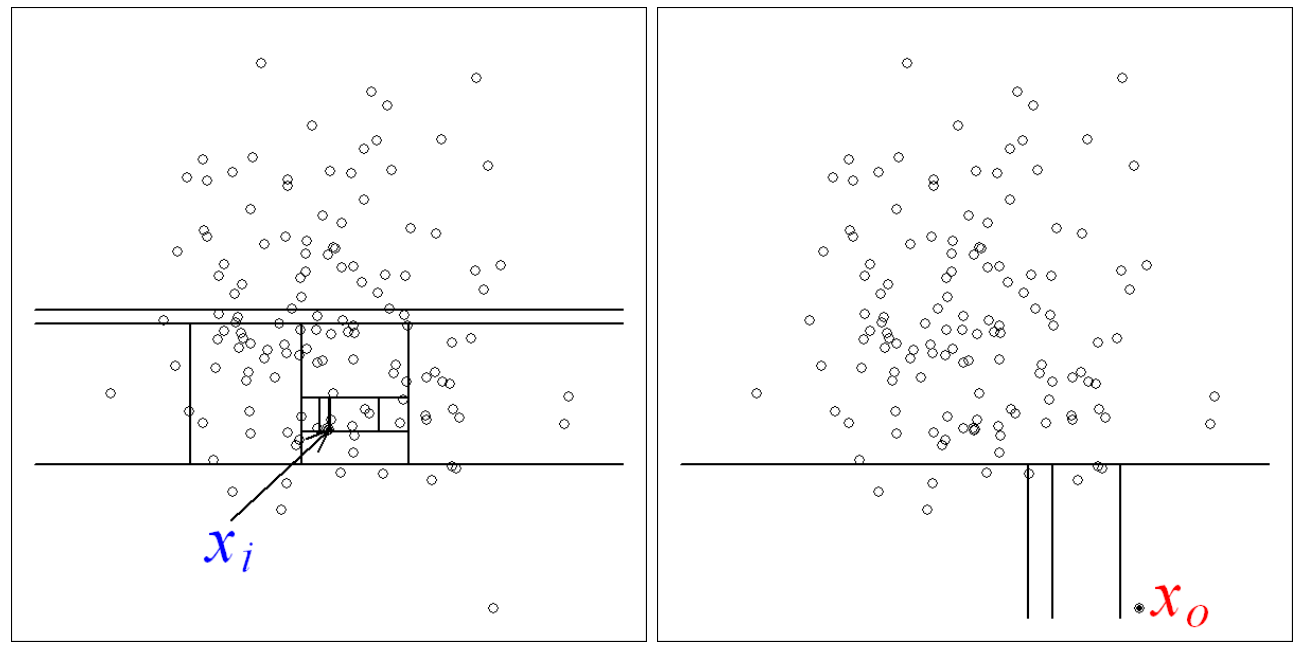
\includegraphics[width=0.80\textwidth]{../fig/chapter2/isolating-a-point.png}
    \captionsource{\textbf{Left}: a normal point $x_i$ requires twelve random partitions to be isolated; \textbf{Right}: an anomaly $x_o$ requires only four partitions to be isolated.}
    {Lui et al. \cite{10.1145/2133360.2133363}}
\end{figure}


\vspace{1em}
\begin{figure}[!ht]
    \label{fig:path-length}
    \centering
    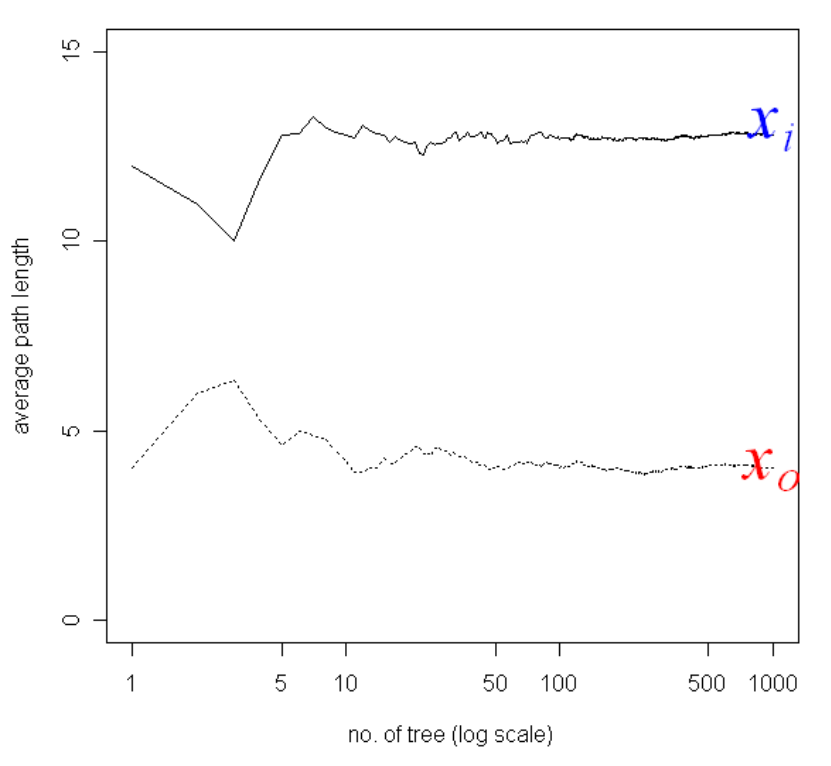
\includegraphics[width=0.50\textwidth]{../fig/chapter2/path-length-for-that-point.png}
    
    \captionsource{Averaged path lengths of $x_i$ and $x_o$ converge when the number of trees increases.}
    {Lui et al. \cite{10.1145/2133360.2133363}}
\end{figure}

\section{Isolation forest algorithm}
\label{sec:iforest-algorithm}

Formally, we can define isolation forest as follows:

\begin{defn}
    \label{defn:isolation-tree}
    (Isolation Tree)
    Let T be a node of an isolation tree.
    T is either an external-node with no child, or an internal-node with one test and exactly two daughter nodes $(T_l, T_r)$.
    A test at node $T$ consists of an attribute $q$ and a split value $p$ such that the test $q < p$ determines the traversal of a data point to either $T_l$ or $T_r$.
    Let X = $\{x_1, ..., x_n\}$ be the given data set of a d-variate distribution.
    A sample of instances X'$\subset$ X is used to build an isolation tree (algorithm~\ref{alg:iTree}).
    We recursively divide X' by randomly selecting an attribute q and a split value p, until either: i) Node has only one instance ii) Or, all data at the node have the same values.
\end{defn}


\begin{defn}
    \label{defn:isolation-forest}
    (Isolation Forest)
    Isolation forest is defined as 4-tuple $(X, t, \psi, S)$ where
    \vspace{-1em}
    \begin{itemize}
        \setlength\itemsep{-1em}
        \item X is input data,
        \item t is number of trees,
        \item $\psi$ is subsampling size and
        \item S is the set of isolation trees.
    \end{itemize}
    \vspace{-1em}
    The elements of set S is constructed (algorithm~\ref{alg:iForest}) by sampling $\psi$ instances from X without replacement.
\end{defn}

\vspace{1em}
\begin{algorithm}[H]
    \caption{$iForest(X,t,\psi)$}\label{alg:iForest}
    \setstretch{1.2}
    \SetAlgoLined
    \KwComplexity{Time - $O(t\psi^2)$, Space - $O(t\psi)$}
    \KwInput{$X$ - input data, $t$ - number of trees, $\psi$ - subsampling size}
    \KwOutput{List of $iTrees$}

    $Forest \: \leftarrow $ EmptyList

    \For {$i = 1$ to $t$}{
        $X' \: \leftarrow \: sampleWithoutReplacement(X,\psi)$

        $Forest.append(iTree(X'))$
    }

    \Return{Forest}
\end{algorithm}

\vspace{1em}
\begin{algorithm}[H]
    \caption{$iTree(X)$}\label{alg:iTree}
    \setstretch{1.2}
    \SetAlgoLined
    \KwComplexity{Time - $O(\psi^2)$, Space - $O(\psi)$}
    \KwInput{$X$ - input data}
    \KwOutput{an $iTree$}

    q $\leftarrow \: RandomChoice(X.attributes)$

    p $\leftarrow \: RandomNumber(X[$splitAttr$].min(), X[$splittAttr$].max())$

    tree $\leftarrow$ Node \{ left $\leftarrow$ None, right $\leftarrow$ None, size $\leftarrow \: X.size$

    \qquad\qquad\qquad splitAttr $\leftarrow$ q, splitVal $\leftarrow$ p\}

    \If{X.size $>$ 1 and X[splitAttr].numUnique() $>$ 1}{
        $X_{l} \: \leftarrow  \: X.where(q < p)$

        $X_{r} \: \leftarrow  \: X.where(q \geq p)$

        tree.left $\leftarrow \: iTree(X_{l})$

        tree.right $\leftarrow \: iTree(X_{r})$
    }

    \Return{tree}
\end{algorithm}
\vspace{1em}

\section{Evaluation}
\label{sec:iforest-evaluation}


\vspace{1em}
\begin{algorithm}[H]
    \caption{$PathLength(x, T, hlim, e)$}\label{alg:PathLength}
    \DontPrintSemicolon
    \setstretch{1.2}
    \SetAlgoLined
    \KwComplexity{Time - $O(t\psi)$, Space - $O(1)$}
    \KwInput{$x$ - input instance, $T$ - an iTree, $hlim$ - height limit, $e$ - current path length to be initialized to zero when called first time}
    \KwOutput{path length of $x$}

    \If{ (T.right is None) and (T.left is none) and (e $\geq$ hlim)}{

        \Return $e + c(T.size)$ \tcp*{c(...) is defined in Equation \ref{eq:average-path-length-of-unsuccessful-searches-bst}}

    }

    $a \: \leftarrow \: T.splitAttr$

    \If{ $x[a] < T.splitVal$}{
        \Return  $PathLength(x, T.left, hlim, e + 1)$
    }
    \Else{
        \Return  $PathLength(x, T.right, hlim, e + 1)$
    }
\end{algorithm}
\pagebreak

In the evaluation stage, a single path length $h(x)$ is derived by counting the number of edges $e$ from the root node to an external node as instance $x$ traverses through an iTree.
When the traversal reaches a predefined height limit $hlim$, the return value is $e$ plus an adjustment $c(size)$ (defined in section~\ref{sec:iforest-anomaly-score}, equation~\ref{eq:average-path-length-of-unsuccessful-searches-bst}).

This adjustment accounts for estimating an average path length of a random sub-tree which could be constructed using data of $size$ beyond the tree height limit.
When $h(x)$ is obtained for each tree of the ensemble, an anomaly score is computed.
The anomaly score and the adjustment $c(size)$ is defined in the next section.

\section{Anomaly Score}
\label{sec:iforest-anomaly-score}

The difficulty in deriving an anomaly score from $h(x)$ is that while the maximum possible height of iTree grows in the order of the subsampling size $\psi$, the average height grows in the order of $log\,\psi$.
When required to visualize or compare path lengths from models of different subsampling sizes, normalization of $h(x)$ by any of the above terms either is not bounded or cannot be directly compared.
Thus, a normalized anomaly score is needed for the aforementioned purposes.

Since iTrees have an equivalent structure to Binary Search Tree, the estimation of average $h(x)$ for external node terminations is the same as that of the unsuccessful searches in BST.

Section 10.3.3 of \cite{10.5555/289373} gives the average path length of unsuccessful searches
in BST as:

\vspace{-2em}
\begin{equation}
    \label{eq:average-path-length-of-unsuccessful-searches-bst}
    \begin{split}
        c(\psi) =  \left\{
        \begin{matrix}
            2H(\psi -1) - 2(\psi -1)/n & \text{for}\: \psi>2,\\
            1 &  \text{for}\: \psi=2,\\
            0 & \text{otherwise.}
        \end{matrix}\right.
    \end{split}
\end{equation}

where $H(i) \approx \ln(i) + 0.5772156649$  (euler's constant), is the harmonic number. As $c(\psi)$ is the average of $h(x)$ given $\psi$, we use it to normalise $h(x)$.
The anomaly score $s$ of an instance $x$ is defined as:

\begin{equation}
    \label{eq:iforest-anomaly-score-for-an-instance}
    s(x,\psi) = 2^{\frac{-E[h(x)]}{c(\psi)}}
\end{equation}

where $E[h(x)]$ is the average of $h(x)$ from a collection of iTrees. 

Anomaly score $s(x,\psi)$ is interpreted as follows:

\begin{enumerate}
    \vspace{-1em}
    \setlength\itemsep{-1em}
    \item if $s \approx 1$, instance is abnormal
    \item if $s \approx 0$, instance is nominal
    \item if $s \approx 0.5$, no distinct anomaly
\end{enumerate}

\vspace{1em}
\begin{figure}[!ht]
    \centering
    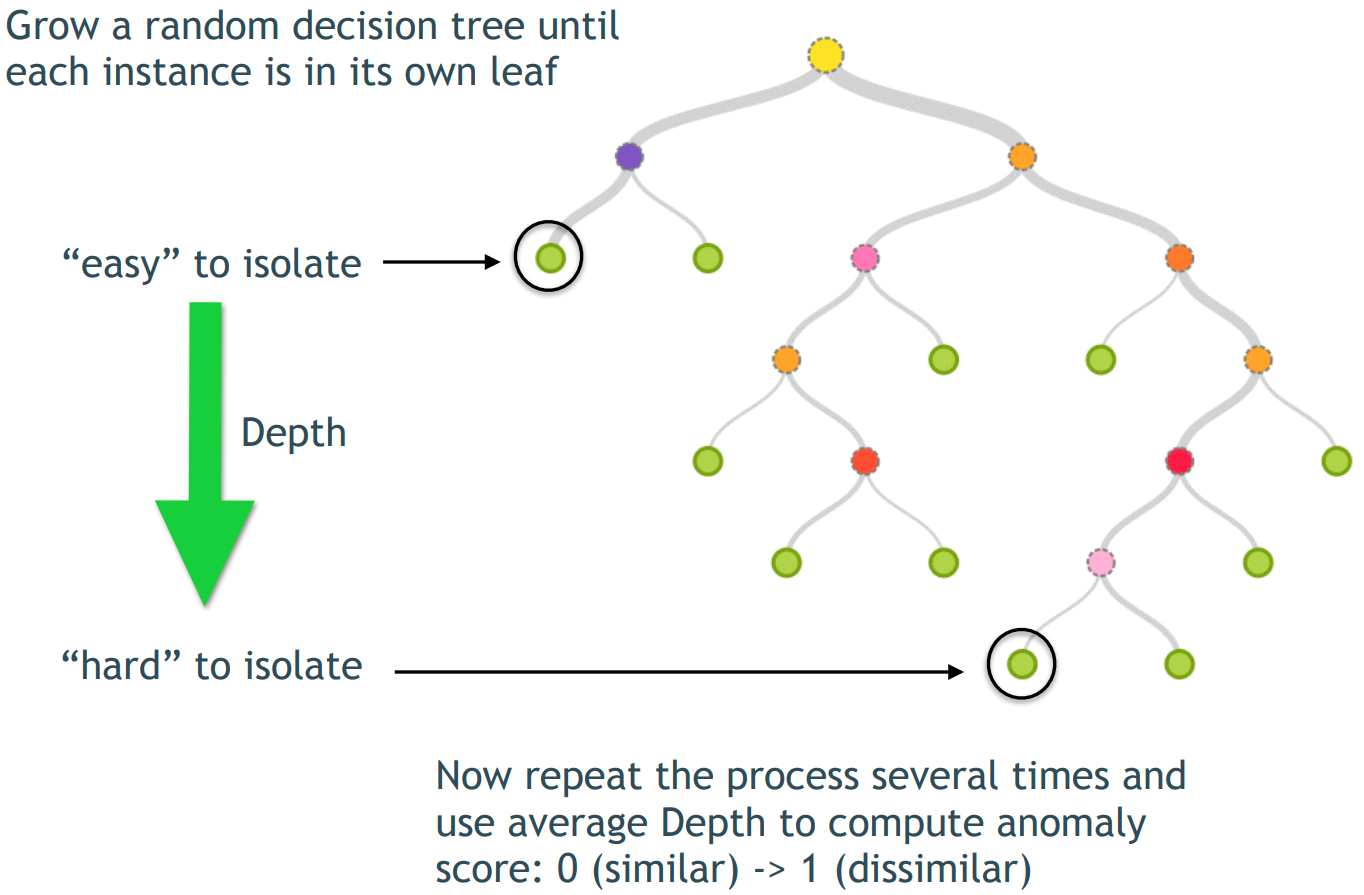
\includegraphics[width=0.80\textwidth]{../fig/chapter2/iforest-visualization.png}
    \captionsource{Isolation forest}
    {\href{https://www.slideshare.net/mlvlc/l14-anomaly-detection}{slideshare.com}}
    \label{fig:iforest-visualization}
\end{figure}

In practical use cases, one has to set a threshold deciding the result.
And finding a good threshold is a very difficult task.
Most of the times the anomalous points' score overlaps with the nominal points' score.

\section{Comparing isolation with distance and density measure}
\label{sec:isolation-vs-distance-density}

Using basic density measures, the assumption is that ‘Normal points occur in dense regions, while anomalies occur in sparse regions’.
Using basic distance measures, the basic assumption is that ‘Normal point is close to its neighbours and anomaly is far from its neighbours’.

There are violations of these assumptions: i) high density and short distance do not always imply normal instances ii) low density and long distance do not always imply anomalies.

\begin{figure}
    \label{fig:high-density-short-distance}
    \centering
    \subfigure[density based method k-NN]{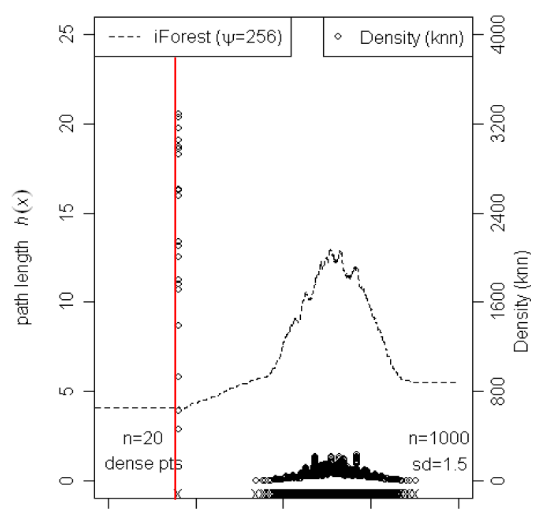
\includegraphics[width=0.4\textwidth]{../fig/chapter2/high-density-short-distances-1.png}}
    \subfigure[distance based method kth-distance]{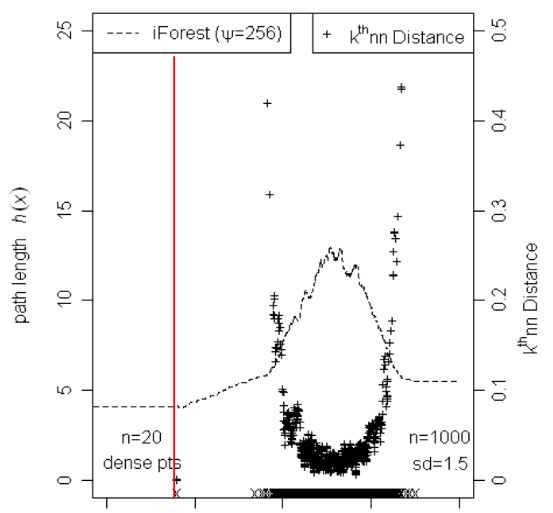
\includegraphics[width=0.4\textwidth]{../fig/chapter2/high-density-short-distances-2.png}}
    \captionsource{High density and short distance do not always imply normal instances.}
    {Lui et al. \cite{10.1145/2133360.2133363}}
\end{figure}

\begin{figure}
    \label{fig:low-density-long-distance}
    \centering
    \subfigure[density based method k-NN]{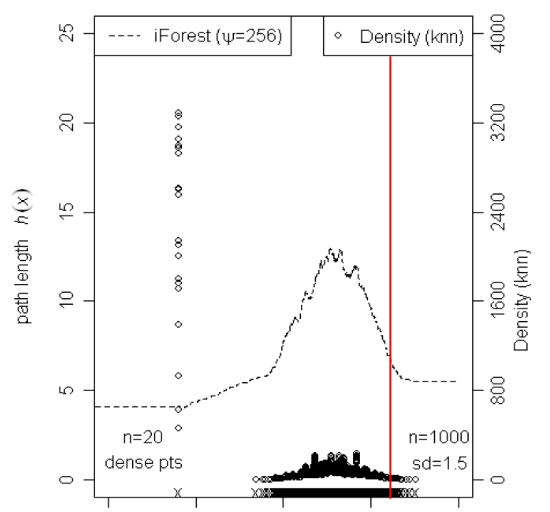
\includegraphics[width=0.4\textwidth]{../fig/chapter2/low-density-long-distances-1.png}}
    \subfigure[distance based method kth-distance]{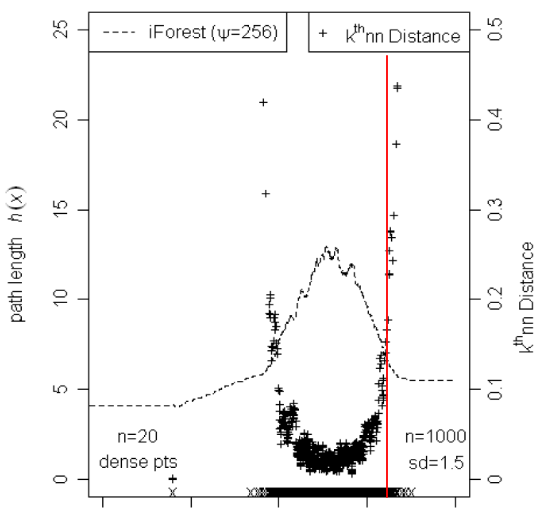
\includegraphics[width=0.4\textwidth]{../fig/chapter2/low-density-long-distances-2.png}}
    \captionsource{Low density and long distance do not always imply anomalies.}
    {Lui et al. \cite{10.1145/2133360.2133363}}
\end{figure}

Isolation forest compares favourably to distance and density  based methods in terms of accuracy and processing time.
Distance and density based suffers immensely in terms of accuracy and processing time because of curse of dimensionality.


Distance based methods also suffers from masking and swamping effect. 
In isolation forest, masking and swamping effects can be managed by adjusting the $hlim$ parameter during evaluation.
Refer section 4.5, 5.3 and 5.4 of Lui et al. \cite{10.1145/2133360.2133363}.


Codes for \href{https://github.com/KishoreKaushal/AnomalyDetection/blob/master/isolationforest/IsolationForest.py}{Isolation Forest} and \href{https://github.com/KishoreKaushal/AnomalyDetection/blob/master/isolationforest/IsolationTree.py}{Isolation Tree} can be found at \href{https://github.com/KishoreKaushal/AnomalyDetection}{this} repository.


\section{Conclusion}
\label{sec:iforest-conclusion}

To conclude, isolation forest is one of the most efficient and accurate methods for anomaly detection.
It outperforms various density and distance based methods like ORCA, DOLPHIN, LOF, ROF, etc and their variants in terms of accuracy and performance.
Still, there are some shortcomings of the isolation forest that we will discuss in next chapter.

